%% ODER: format ==         = "\mathrel{==}"
%% ODER: format /=         = "\neq "
%
%
\makeatletter
\@ifundefined{lhs2tex.lhs2tex.sty.read}%
  {\@namedef{lhs2tex.lhs2tex.sty.read}{}%
   \newcommand\SkipToFmtEnd{}%
   \newcommand\EndFmtInput{}%
   \long\def\SkipToFmtEnd#1\EndFmtInput{}%
  }\SkipToFmtEnd

\newcommand\ReadOnlyOnce[1]{\@ifundefined{#1}{\@namedef{#1}{}}\SkipToFmtEnd}
\DeclareFontFamily{OT1}{cmtex}{}
\DeclareFontShape{OT1}{cmtex}{m}{n}
  {<5><6><7><8>cmtex8
   <9>cmtex9
   <10><10.95><12><14.4><17.28><20.74><24.88>cmtex10}{}
\DeclareFontShape{OT1}{cmtex}{m}{it}
  {<-> ssub * cmtt/m/it}{}
\newcommand{\texfamily}{\fontfamily{cmtex}\selectfont}
\DeclareFontShape{OT1}{cmtt}{bx}{n}
  {<5><6><7><8>cmtt8
   <9>cmbtt9
   <10><10.95><12><14.4><17.28><20.74><24.88>cmbtt10}{}
\DeclareFontShape{OT1}{cmtex}{bx}{n}
  {<-> ssub * cmtt/bx/n}{}
\newcommand{\tex}[1]{\text{\texfamily#1}}	% NEU

\newcommand{\Sp}{\hskip.33334em\relax}


\newcommand{\Conid}[1]{\mathit{#1}}
\newcommand{\Varid}[1]{\mathit{#1}}
\newcommand{\anonymous}{\kern0.06em \vbox{\hrule\@width.5em}}
\newcommand{\plus}{\mathbin{+\!\!\!+}}
\newcommand{\bind}{\mathbin{>\!\!\!>\mkern-6.7mu=}}
\newcommand{\rbind}{\mathbin{=\mkern-6.7mu<\!\!\!<}}% suggested by Neil Mitchell
\newcommand{\sequ}{\mathbin{>\!\!\!>}}
\renewcommand{\leq}{\leqslant}
\renewcommand{\geq}{\geqslant}

%mathindent has to be defined
\@ifundefined{mathindent}%
  {\newdimen\mathindent\mathindent\leftmargini}%
  {}%

\def\resethooks{%
  \global\let\SaveRestoreHook\empty
  \global\let\ColumnHook\empty}
\newcommand*{\savecolumns}[1][default]%
  {\g@addto@macro\SaveRestoreHook{\savecolumns[#1]}}
\newcommand*{\restorecolumns}[1][default]%
  {\g@addto@macro\SaveRestoreHook{\restorecolumns[#1]}}
\newcommand*{\aligncolumn}[2]%
  {\g@addto@macro\ColumnHook{\column{#1}{#2}}}

\resethooks

\newcommand{\onelinecommentchars}{\quad-{}- }
\newcommand{\commentbeginchars}{\enskip\{-}
\newcommand{\commentendchars}{-\}\enskip}

\newcommand{\visiblecomments}{%
  \let\onelinecomment=\onelinecommentchars
  \let\commentbegin=\commentbeginchars
  \let\commentend=\commentendchars}

\newcommand{\invisiblecomments}{%
  \let\onelinecomment=\empty
  \let\commentbegin=\empty
  \let\commentend=\empty}

\visiblecomments

\newlength{\blanklineskip}
\setlength{\blanklineskip}{0.66084ex}

\newcommand{\hsindent}[1]{\quad}% default is fixed indentation
\let\hspre\empty
\let\hspost\empty
\newcommand{\NB}{\textbf{NB}}
\newcommand{\Todo}[1]{$\langle$\textbf{To do:}~#1$\rangle$}

\EndFmtInput
\makeatother
%
%
%
%
%
%
% This package provides two environments suitable to take the place
% of hscode, called "plainhscode" and "arrayhscode". 
%
% The plain environment surrounds each code block by vertical space,
% and it uses \abovedisplayskip and \belowdisplayskip to get spacing
% similar to formulas. Note that if these dimensions are changed,
% the spacing around displayed math formulas changes as well.
% All code is indented using \leftskip.
%
% Changed 19.08.2004 to reflect changes in colorcode. Should work with
% CodeGroup.sty.
%
\ReadOnlyOnce{polycode.fmt}%
\makeatletter

\newcommand{\hsnewpar}[1]%
  {{\parskip=0pt\parindent=0pt\par\vskip #1\noindent}}

% can be used, for instance, to redefine the code size, by setting the
% command to \small or something alike
\newcommand{\hscodestyle}{}

% The command \sethscode can be used to switch the code formatting
% behaviour by mapping the hscode environment in the subst directive
% to a new LaTeX environment.

\newcommand{\sethscode}[1]%
  {\expandafter\let\expandafter\hscode\csname #1\endcsname
   \expandafter\let\expandafter\endhscode\csname end#1\endcsname}

% "compatibility" mode restores the non-polycode.fmt layout.

\newenvironment{compathscode}%
  {\par\noindent
   \advance\leftskip\mathindent
   \hscodestyle
   \let\\=\@normalcr
   \let\hspre\(\let\hspost\)%
   \pboxed}%
  {\endpboxed\)%
   \par\noindent
   \ignorespacesafterend}

\newcommand{\compaths}{\sethscode{compathscode}}

% "plain" mode is the proposed default.
% It should now work with \centering.
% This required some changes. The old version
% is still available for reference as oldplainhscode.

\newenvironment{plainhscode}%
  {\hsnewpar\abovedisplayskip
   \advance\leftskip\mathindent
   \hscodestyle
   \let\hspre\(\let\hspost\)%
   \pboxed}%
  {\endpboxed%
   \hsnewpar\belowdisplayskip
   \ignorespacesafterend}

\newenvironment{oldplainhscode}%
  {\hsnewpar\abovedisplayskip
   \advance\leftskip\mathindent
   \hscodestyle
   \let\\=\@normalcr
   \(\pboxed}%
  {\endpboxed\)%
   \hsnewpar\belowdisplayskip
   \ignorespacesafterend}

% Here, we make plainhscode the default environment.

\newcommand{\plainhs}{\sethscode{plainhscode}}
\newcommand{\oldplainhs}{\sethscode{oldplainhscode}}
\plainhs

% The arrayhscode is like plain, but makes use of polytable's
% parray environment which disallows page breaks in code blocks.

\newenvironment{arrayhscode}%
  {\hsnewpar\abovedisplayskip
   \advance\leftskip\mathindent
   \hscodestyle
   \let\\=\@normalcr
   \(\parray}%
  {\endparray\)%
   \hsnewpar\belowdisplayskip
   \ignorespacesafterend}

\newcommand{\arrayhs}{\sethscode{arrayhscode}}

% The mathhscode environment also makes use of polytable's parray 
% environment. It is supposed to be used only inside math mode 
% (I used it to typeset the type rules in my thesis).

\newenvironment{mathhscode}%
  {\parray}{\endparray}

\newcommand{\mathhs}{\sethscode{mathhscode}}

% texths is similar to mathhs, but works in text mode.

\newenvironment{texthscode}%
  {\(\parray}{\endparray\)}

\newcommand{\texths}{\sethscode{texthscode}}

% The framed environment places code in a framed box.

\def\codeframewidth{\arrayrulewidth}

\newenvironment{framedhscode}%
  {\parskip=\abovedisplayskip\par\noindent
   \hscodestyle
   \arrayrulewidth=\codeframewidth
   \tabular{@{}|p{\linewidth-2\arraycolsep-2\arrayrulewidth-2pt}|@{}}%
   \hline\framedhslinecorrect\\{-1.5ex}%
   \let\endoflinesave=\\
   \let\\=\@normalcr
   \(\pboxed}%
  {\endpboxed\)%
   \framedhslinecorrect\endoflinesave{.5ex}\hline
   \endtabular
   \parskip=\belowdisplayskip\par\noindent
   \ignorespacesafterend}

\newcommand{\framedhslinecorrect}[2]%
  {#1[#2]}

\newcommand{\framedhs}{\sethscode{framedhscode}}

% The inlinehscode environment is an experimental environment
% that can be used to typeset displayed code inline.

\newenvironment{inlinehscode}%
  {\(\def\column##1##2{}%
   \let\>\undefined\let\<\undefined\let\\\undefined
   \newcommand\>[1][]{}\newcommand\<[1][]{}\newcommand\\[1][]{}%
   \def\fromto##1##2##3{##3}%
   \def\nextline{}}{\) }%

\newcommand{\inlinehs}{\sethscode{inlinehscode}}

% The joincode environment is a separate environment that
% can be used to surround and thereby connect multiple code
% blocks.

\newenvironment{joincode}%
  {\let\orighscode=\hscode
   \let\origendhscode=\endhscode
   \def\endhscode{\def\hscode{\endgroup\def\@currenvir{hscode}\\}\begingroup}
   %\let\SaveRestoreHook=\empty
   %\let\ColumnHook=\empty
   %\let\resethooks=\empty
   \orighscode\def\hscode{\endgroup\def\@currenvir{hscode}}}%
  {\origendhscode
   \global\let\hscode=\orighscode
   \global\let\endhscode=\origendhscode}%

\makeatother
\EndFmtInput
%

\chapter{Background} \label{ch:background}
In this chapter, we briefly present the background needed to read the remainder of this thesis.
We briefly discuss various forms of the $\lambda$-calculus, which we use to reason about functional hardware descriptions.
First, we discuss the untyped $\lambda$-calculus.
Second, we discuss the addition of a simple type system, leading to the simply typed $\lambda$-calculus.
Finally, we discuss the type system of Damas-Milner, which includes polymorphism and constraints, both of which are important for the development of our own type system.

\section{The untyped $\lambda$-calculus}
The untyped $\lambda$-calculus is a minimal algebraic structure, which is used to represent function abstraction and function application.
Within the untyped $\lambda$-calculus, every value is considered a function.
Church has shown through Church-numerals that numbers can be encoded in terms of function application and abstraction.
Function application and abstraction also make it possible to encode booleans, pairs and lists.
All this is possible despite the untyped $\lambda$-calculus comprising of just three terms:
\begin{itemize*}
 \item variable
 \item abstraction
 \item application.
\end{itemize*}

These terms can be used to create expressions as indicated by the following grammar:
\begin{changemargin}{1cm}{0cm}
\begin{expansionno}{text only}
\begin{tabular}{l p{1cm} lr}
e       & $\Coloneqq$ &           &\textit{expressions:}\\
        & |     & x              &\textit{(variable)}\\
        & |     & $\lambda$x.e   &\textit{(abstraction)}\\
        & |     & e e            &\textit{(application)}\\
\end{tabular}
\end{expansionno}
\end{changemargin}

Using the above grammar, we can define functions through abstraction, and apply functions to other functions.
For instance, the identity function is a combination of abstraction and a variable: $\lambda x.x$.
Application to an expression $e$ then allows a reduction step: $(\lambda x.x) e$ can be reduced to simply $e$.
This reduction step is called $\beta$-reduction, which represents the computational aspect of the $\lambda$-calculus.
Various reduction strategies exists such as \textit{normal order reduction}, \textit{call-by-name}, \textit{call-by-value} and \textit{call-by-need} which specify the exact conditions under which a reduction can take place.
For a more detailled account see ``The lambda calculus: Its syntax and semantics''\cite{barendregt1985lambda}.
Whenever an expression can be reduced, it is called a redex, short for \textit{reducible expression}.
Whenever an expression cannot be reduced, it has reached its \textit{normal form}.
The normal form of an expression depends on the reduction strategy used.

We can imagine expressions as representing a tree structure.
For instance, we can apply the identity function to the identity function as expressed by $(\lambda x.x) (\lambda y.y)$.
This expression represents a tree of function abstraction and application, as shown by figure \ref{fig:tree}.
This structure is called the abstract syntax tree.

\begin{figure}[h]
\centering
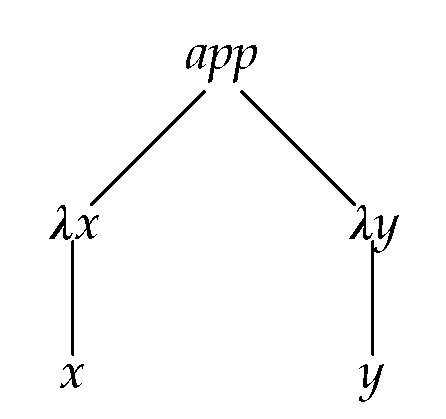
\includegraphics[width=0.3\textwidth]{images/tree}
\caption{Tree structure of the expression $(\lambda x.x) (\lambda y.y)$} \label{fig:tree}
\end{figure}

The untyped $\lambda$-calculus is a rewriting system. 
Redexes are rewritten by replacing free occurences of variables in an expression with another expression.
For instance, the expression $e = (\lambda x.e_1) \: e_2$ can be rewritten as $e = [x \mapsto e_2] e_1$, where $[x \mapsto e_2]$ replaces all free occurences of $x$ in $e_1$ with $e_2$.
A free occurence of a variable is one which is not bound by any abstraction. 
In $e$, the variable $x$ used in $e_1$ refers to the binder $\lambda x$, and as such may be replaced by $e_2$ when applying the substitution $[x \mapsto e_2] e_1$.
When replacing free occurences of $x$ in $e_1$, we have to be careful of \textit{shadowing}, where $e_1$ itself contains an abstraction of $x$ again.
The inner $\lambda$-abstraction ``shadows'' the outer $\lambda$-abstraction.
As a result, not every occurence of $x$ may be replaced within $e_1$, but only the free occurences of $x$.

As shown, the untyped $\lambda$-calculus provides a minimal amount of structure through its grammar. 
In the next section we discuss the simply-typed $\lambda$-calculus, which provides additional structure through its \textit{type system}.

\section{Simply-typed $\lambda$-calculus}
Within the untyped $\lambda$-calculus, a number of expressions are considered valid, but when reduced using $\beta$-reduction will never reach a normal-form.
A normal form is a state where an expression can no longer be rewritten; the computation is finished.
For instance, the expression $\Omega = (\lambda x. x x) (\lambda x. x x)$ will never evaluate to a normal-form.
The expression $Y = \lambda f.( \lambda x.f (x x)) (\lambda x.f (x x))$, named Curry's Y-combinator, allows us to define basic recursion, which also has the ability to never evaluate to a normal-form.

To disallow these non-normalising functions, the simply typed $\lambda$-calculus introduces a type system, where every term has a well-defined type.
The simply typed $\lambda$-calculus is strongly normalizing.
Strongly normalizing implies that every valid expression will reduce to a normal form without exception.
In practice, this is often considered too strict, which is why a fixpoint-combinator can be introduced as a \textit{primitive}.
A primitive is, like the terms of the untyped $\lambda$-calculus, part of the definition of the language.

Since every valid expression reduces to a normal form, every valid expression is known to be terminating, given finite inputs.
As a result, the simply-typed $\lambda$-calculus is \textit{not} turing-complete.
We introduce the grammar of the simply-typed $\lambda$-calculus below, or $\lambda^\rightarrow$ for short.

\begin{definitiontitled}[text only,float]{Grammar of $\lambda^{\rightarrow}$}{def:lambda}
\begin{changemargin}{-0.5cm}{0cm}
\begin{minipage}[b]{0.50\linewidth}
\begin{tabular}{lclr}
e       & $\Coloneqq$ &                             & \textit{expressions:} \\
        & |    & x                                 & \textit{(variable)} \\
        & |    & $\lambda$ x:$\tau$.e              & \textit{(abstraction)} \\
        & |    & e e                               & \textit{(application)} \\
        & |    & c                                 & \textit{(constant)} \\
        & |    & \textbf{let} x = e \textbf{in} e  & \textit{(let binding)} \\
\\
c       & $\Coloneqq$ &                             & \textit{primitive literals} \\
        & |    & true                              & \textit{(Boolean true)} \\
        & |    & false                             & \textit{(Boolean false)} \\
        & |    & n $\in \mathbb{Z}$                & \textit{(Integer literals)} \\
\end{tabular}
%\captionof{table}{Definition of $\lambda$ with explicit data.}
\end{minipage}
\begin{minipage}[b]{0.40\linewidth}
\begin{tabular}{lclr}
$\tau$  & $\Coloneqq$ &                             & \textit{types:} \\
        & |     & $\tau \rightarrow \tau$          & \textit{(function type)} \\
        & |     & T                                & \textit{(base type)} \\
\\
T       & $\Coloneqq$ &                             & \textit{base types:} \\
        & |     & Bool                             & \textit{(Boolean type)} \\
        & |     & Int                              & \textit{(Integer type)} \\
\\
$\Gamma$& $\Coloneqq$ &                             & \textit{contexts:} \\
        & |     & $\emptyset$                      & \textit{(empty context)} \\
        & |     & $\Gamma$,x:T                     & \textit{(term variable binding)} \\
\end{tabular}
%\captionof{table}{Definition of $\lambda_{\rightarrow}$}
\end{minipage}
\end{changemargin}
\end{definitiontitled}

This definition shows the addition of a type $\tau$ to the abstraction expression.
Variables introduced through $\lambda$-abstraction need to have a type annotation, in order for the system to be able to construct the correct function type.
Types have one constructor, namely $\rightarrow$, which constructs a function type from two other types.
Types need to be finite, meaning construction of a type must always terminate.
As a result, every type must, at some point, use base types in its definition.

$\lambda^\rightarrow$ can not express polymorphism.
For instance, the general form of the identity function in the untyped $\lambda$-calculus ($\lambda x.x$), is not valid in $\lambda^\rightarrow$, as $x$ must have a type.
Whenever $x$ has a type, such as in $\lambda x:Int.x$, we can derive the type of the expression.
The $\lambda$-abstraction introduces the $\rightarrow$ constructor, which allows us to create function types using base types.
The function $(\lambda x:Int.x)$ has type $Int \rightarrow Int$, since the type of the result of the identity function has the same type as the function argument.
We will revisit polymorphism in section \ref{sec:polymorphiclambda}.

The type system of $\lambda^\rightarrow$ is not complete without typing rules.
Typing rules express the relation between types and expressions, and in particular define which expressions are \textit{valid} and which are not.
The nature of the typing rules for $\lambda^\rightarrow$ also makes it possible to \textit{(re)construct} the the types from (partial) type information.
We will explain the typing rules of $\lambda^\rightarrow$ next, where we we also explain the meaning of the context $\Gamma$ as introduced by definition \ref{def:lambda}.

\subsection{Typing rules}
In this section we present the typing rules of $\lambda^\rightarrow$, using the commonly used Gentzen style of the sequent calculus\cite{gentzen1935untersuchungen}.
For every valid expression $e$ in $\lambda^\rightarrow$, a single rule expresses the relation between the expression and the type of the expression.
Using these rules, a proof can be constructed for any valid expression $e$ in $\lambda^\rightarrow$, by (de)-constructing the expression using the typing rules.
When a proof cannot be constructed, then the expression is considered invalid.

We use $\tau$ and $\rho$ to range over types.
As is customary in type theory, we use $\Gamma$ to represent the \textit{context} or \textit{type environment}.
$\Gamma$ is a set of pairs, which expresses the relation between \textit{variable names} and \textit{types}, as shown by definition \ref{def:lambda}.
The type environment is needed in order to make judgements based on the context an expression is used in.
For instance, the expression $x + 1$ cannot be typed when nothing is known about $x$. 
We use $\Gamma$ to provide the context in which we can make a statement about $x+1$. 
If $\Gamma = \{ x : \textit{Int}, + : \textit{Int} \rightarrow \textit{Int} \rightarrow \textit{Int} \}$ and we assume that the literal $1$ has type \textit{Int}, then the entire expression would have type \textit{Int} as well.
However, we can only make this judgement when we know the context $\Gamma$ in which the statement $x+1$ is used.

In the typing rules, statements about the context are made explicit by use of the \textit{turnstile} ($\vdash$) symbol.
For instance, $\Gamma \vdash x : \tau$ indicates that the type of $x$ is $\tau$, which is derived from the context $\Gamma$.
The turnstile indicates derivability; we can derive $x : \tau$ from $\Gamma$.
As shown by the typing rules of definition \ref{def:typerulelambda}, typing rules consist of of two parts: the \textit{premise} of the rule, and the \textit{conclusion}.
The premise is separated from the conclusion by a horizontal line, with the premise(s) above the line, while the conclusion is written below the line.

\begin{definitiontitled}[text only]{Typing Rules for $\lambda^\rightarrow$}{def:typerulelambda}
\begin{tabularx}{\textwidth}{ c l X c r}
$ \displaystyle
  \frac
    { }
    { \Gamma, x : \tau \vdash x : \tau }
$ & 
T-Var
&
&
$ \displaystyle
  \frac
    { }
    { c : T }
$
&
T-Const
\\
\\
$ \displaystyle
  \frac
    { \Gamma,x:\rho \vdash e : \tau }
    { \Gamma \vdash \lambda x:\rho.e : \rho \rightarrow \tau}
$
&
T-Abs
&
&
$ \displaystyle
  \frac
    { \Gamma \vdash e_1 : \rho \rightarrow \tau \quad \Gamma \vdash e_2 : \rho }
    { \Gamma \vdash e_1 \: e_2 : \tau }
$
& 
T-App
\\
\end{tabularx}\\
\\

\begin{tabularx}{\textwidth}{X r l X}
 &
$ \displaystyle
  \frac
    { \Gamma \vdash e_1 : \rho \quad \Gamma,x:\rho \vdash e_2 : \tau}
    { \Gamma \vdash \textbf{let } x=e_1 \textbf{ in } e_2 : \tau}
$ 
& 
T-Let
&
\\
\end{tabularx}
\end{definitiontitled}

As shown, both the rules T-Var and T-Const are trivial.
Given a literal ``true'', ``false'' or a natural number, we can conclude that it would have either the type \textit{Bool} or \textit{Int}. 
The rule T-Var is slightly less trivial.
The conclusion $\Gamma, x : \tau \vdash x : \tau$ defines that, whatever the context $\Gamma$ is, when we add $x : \tau$ to it, we can conclude that $x$ does indeed have type $\tau$.
While it may seem that both of these rules can always be applied because there is a lack of a premise, it is really only the case for T-Const.
We can only derive $x : \tau$ in T-Var when $x : \tau$ is part of the context $\Gamma$.
This means that the statement $x + 1$, with the empty context $\varnothing$, does not have a derivable type.
The variable $x$ must be introduced by $\lambda$-abstraction, as defined in the following rule, T-Abs.

The rule T-Abs shows the relation between abstraction and the function type constructor $\rightarrow$.
The context $\Gamma$ is extended with $x:\rho$ when deriving the expression $e$ where $x$ is abstracted from.
From the extended context $\Gamma$ we then derive $e$ has type $\tau$.
When the entire premise $\Gamma, x : \rho \vdash e : \tau$ holds, we derive from the \textit{non-extended} $\Gamma$, that $\lambda x:\rho.e$ has type $\rho \rightarrow \tau$.
With the T-Abs rule, we show how abstraction \textit{introduces} a function type.

Conversely, the T-Abs rule eliminates the $\rightarrow$ type constructor.
The rule T-App has two premises, where both $e_1$ and $e_2$ are derived to have the types $\rho \rightarrow \tau$ and $\rho$ respectively.
Here, when we mention $\rho$, we mean the \textit{same} type in both premises.
This means that the T-Abs rule can only be applied when the left-most expression $e_1$ of application has a function type.
Moreover, the type of the right-most expression $e_2$ must match the argument of the type of $e_1$.
When these premises hold, we may derive $e_1 \: e_2 : \tau$ from the same context $\Gamma$.

Finally, the T-Let rule defines two premises must hold, in order to derive $\textbf{let } x = e_1 \textbf{ in } e_2$ to have type $\tau$.
First, we use the context $\Gamma$ to derive the type of $e_1$ to be $\rho$.
Secondly, we add the type binding $x : \rho$ to $\Gamma$ in order to derive the type of $e_2$.
The type of $x$ must be added to $\Gamma$, as $x$ is (probably) referenced within $e_2$, so in order to derive the type of $e_2$, the context must have that information available.
When both these premises hold, then the entire let-statement has type $\tau$.
As the simply typed $\lambda$-calculus has no polymorphism the use of the let-binding is limited.
In the next section we give an introduction to let-polymorphism and constraint-based typing.

\section{Polymorphic $\lambda$-calculus} \label{sec:polymorphiclambda}
In the simply-typed $\lambda$-calculus, no polymorphic functions can be defined.
A polymorphic function can be seen as a \textit{family} of functions, of which an instance is chosen depending on the context which it is used in.
As a trivial example, consider the identity function $\lambda x.x$.
The identity function in the untyped $\lambda$-calculus does not have a notion of types, and can therefor be applied to any value.
This is not the case in the simply-typed $\lambda$-calculus, but we can define the set of all functions which \textit{share} the definition of the identity function under type-erasure.
Both the functions $(\lambda x : \textit{Int}. x) : \textit{Int} \to \textit{Int}$ and $(\lambda x : \textit{Bool}.x) : \textit{Bool} \to \textit{Bool}$ share the same definition.
While this makes intuitive sense, it is not a trivial problem for a type system to solve.
\citeauthor{wand1987simple} defines\cite{wand1987simple} the problem of polymorphism as ``Given a term of the untyped $\lambda$-calculus, to find all terms of the typed $\lambda$-calculus which yield the given term when the type information on bound variables is deleted.''
In effect, when we have an expression of the untyped $\lambda$-calculus, we try to find the \textit{family} of valid types belonging to that expression.

To show how this is done, we first extend the grammar of $\lambda^\rightarrow$.
Secondly, we introduce polytypes, which allow us to reason about polymorphic types.
Using polytypes, we define what constitutes the most general type of an expression, known as the principal type. 
Finally, using principal types and polytypes, we show how the process of type-checking is split in two by using \textit{constraints}.
To do so, we focus on the well-known ``Damas-Milner''\cite{damas1982principal} type reconstruction algorithm, which is also known as the ``Hindley-Milner'' or ``Damas-Hindley-Milner'' type reconstruction algorithm.
%We also briefly look at the type system of ``Parameterized Hindley-Milner''\cite{odersky1999type}, also known as HM(X), to show how constraints can be represented in typing rules.
%HM(X) is considered\cite{pierce2005advanced} an extension of the type system of Damas-Milner, which is why our discussion of it will only be very brief.

\subsection{Principal Types}
We focus on principal types first.
We extend the grammar of $\lambda^\rightarrow$ with type variables.
This leads to the grammar we call $\lambda_{DM}$, which is shown by definition \ref{def:lambdaconstraint}.
The rest of the grammar is identical to $\lambda^\rightarrow$ from definition \ref{def:typerulelambda}.
As we are introducing polymorphism to the simply typed $\lambda$-calculus, we need a mechanism to introduce polymorphic functions.
For this we use \textit{let-polymorphism} as introduced\cite{milner1978theory} by \citeauthor{milner1978theory}. 
There, let-bindings are used to introduce polymorphic functions, which can be used multiple times within the body of the let-binding, regardless of possible conflicting types between each instance.
We discuss the idea of let-polymorphism in greater detail later in this section.

\begin{definitiontitled}[text only,float]{Grammar of $\lambda_{DM}$ (Extended from definition \ref{def:lambda}).}{def:lambdaconstraint}
\begin{tabular}{lclr}
$\tau$  & $\Coloneqq$ & $\alpha$          &\textit{(type variable)}\\
        & |          & $\ldots$          & \\
\\
$e$     & $\Coloneqq$ & $\lambda x.e$     &\textit{(abstraction)} \\
        & |           & \ldots           & \\
\end{tabular}
\end{definitiontitled}

Aside from using $\alpha$ for type variables, we also use $\beta$ when two type variables are distinctly different.
Type variables in $\lambda_{DM}$ are \textit{monomorphic}, meaning a type variable can only refer to a single type.
Moreover, without further modification, all type variables are \textit{free} variables, as they are not bound to abstraction like term variables in the $\lambda$-calculus.
Type variables are used in \textit{polytypes}\footnote{Some authors, such as \citeauthor{milner1978theory}, prefer to use the term \textit{type scheme}. Here, we use the term polytype.}, shown by definition \ref{def:typescheme}.
Polytypes make it possible to introduce \textit{polymorphism} using monomorphic type variables. 

\begin{definitiontitled}[text only,float]{Polytypes}{def:typescheme}
A polytype $\sigma$ is defined by universal quantification over a finite number of type variables:
\[
\sigma = \forall \alpha_0,\alpha_1, \ldots, \alpha_n. \tau \quad (n \ge 0)
\]
, where the type variables $\alpha_0$ to $\alpha_n$ are considered bound within $\tau$.
\end{definitiontitled}

Polytypes consist of universal quantification over type variables.
The type variables used by universal quantification are bound within the polytype $\sigma$.
In the polytype $\sigma = \forall \varnothing.\tau$, the polytype $\sigma$ is equal to the type $\tau$.
Whenever a substitution of the form $[\alpha \mapsto \rho]$ is applied to a polytype $\sigma$, the resulting type is called an \textit{instance} of $\sigma$.
Similarly, a \textit{set} of substitutions $S$ may be applied to $\sigma$.

We can use polytypes to define polymorphic functions.
For instance, the identity function $\lambda x.x$ is polymorphic when it has the associated polytype $\sigma = \forall \alpha. \alpha \rightarrow \alpha$.
When applied to a value, for instance $1 : \textit{Int}$, the substitution $[\alpha \mapsto Int]$ can be applied to $\sigma$, leading to the type instance $\sigma = \forall \varnothing. \textit{Int} \rightarrow \textit{Int}$.

As shown, we can create an instance of a polytype by applying a substitution to a polytype.
Given the identity function, there exist many different substitutions to create type instances of the associated polytype.
For instance, the identity function, when associated with polytype $\sigma = \forall \alpha. \alpha \rightarrow \alpha$, can be instantiated using the substitutions $[\alpha \mapsto \textit{Bool}]$, $[\alpha \mapsto \textit{Int}]$, or even $[\alpha \mapsto (\textit{Int} \rightarrow \textit{Bool})]$ and other variations.
Given that many substitutions exists, the principal type is defined informally as the type which is least constricting, but is still a valid type.
That is, the principal type $\tau$ of an expression $e$, is the type to which any set of substitutions may be applied, assuming the set of substitutions lead to a valid type $\tau'$ of $e$.

\begin{definitiontitled}[text only,float]{Principal Types}{def:principal}
Given a type $\tau$, associated with a polytype $\sigma = \forall \alpha_0, \alpha_1 \ldots \alpha_n. \tau$ of an expression $e$, then $\tau$ is the principal type of $e$ iff:
\begin{enumerate}
 \item the type $\tau$ holds under the empty context, that is, $\varnothing \vdash e : \tau$;
 \item $\forall \tau'. \varnothing \vdash e : \tau' \Rightarrow \exists S.\tau' = S\tau$, that is, for all valid types $\tau'$ of $e$, there exists a set of substitutions $S$, such that $\tau$ can be turned into $\tau'$.
\end{enumerate}
\end{definitiontitled}

In some of the literature the binary relation $\sqsubseteq$ is defined as well.
This relation is used to express an ordering in polytypes.
Given two polytypes $\sigma' \sqsubseteq \sigma$ defines $\sigma'$ to be at least as constricting as $\sigma$.
For instance, given $(\sigma' = \forall \alpha. \textit{Int} \to \alpha)$ and $(\sigma = \forall \alpha,\beta. \beta \to \alpha)$, the relation $\sigma' \sqsubseteq \sigma$ holds.
Similarly, $\sigma \sqsubseteq \sigma$ holds, as $\sigma$ is at least as constricting as itself.

\begin{definitiontitled}[text only]{Typing Rules for $\lambda_{DM}$}{def:dmrules}
\begin{tabularx}{\textwidth}{ c l X c r}
$ \displaystyle
  \frac
    { \Gamma(x) = \sigma }
    { \Gamma \vdash x : \sigma }
$ & 
DM-Var
&
&
$ \displaystyle
  \frac
    { }
    { \varnothing \vdash c : T }
$
&
DM-Const
\\
\\
$ \displaystyle
  \frac
    { \Gamma,x:\rho \vdash e : \tau }
    { \Gamma \vdash \lambda x:\rho.e : \rho \rightarrow \tau}
$
&
DM-Abs
&
&
$ \displaystyle
  \frac
    { \Gamma \vdash e_1 : \rho \rightarrow \tau \quad \Gamma \vdash e_2 : \rho }
    { \Gamma \vdash e_1 \: e_2 : \tau }
$
& 
DM-App
\\
\\
$ \displaystyle
  \frac
  { \Gamma \vdash t : \sigma \quad \alpha \notin \textit{ftv}(\Gamma) }
  { \Gamma \vdash e : \forall \alpha.\sigma }
$
&
DM-Gen
& 
& 
$ \displaystyle
  \frac
  { \Gamma \vdash e : \sigma \quad \sigma' \sqsubseteq \sigma }
  { \Gamma \vdash e : \forall \alpha.\sigma' }
$
&
DM-Inst
\\
\end{tabularx}\\
\\

\begin{tabularx}{\textwidth}{X r l X}
 &
$ \displaystyle
  \frac
    { \Gamma \vdash e_1 : \sigma \quad \Gamma,x:\sigma \vdash e_2 : \tau}
    { \Gamma \vdash \textbf{let } x=e_1 \textbf{ in } e_2 : \tau}
$ 
& 
DM-Let
&
\\
\end{tabularx}
\end{definitiontitled}

Using principal types, we define the typing rules of the Damas-Milner type system in definition \ref{def:dmrules}.
Most of the rules of the Damas-Milner type system are straightforward.
The rules DM-Abs and DM-App are exactly the same as the rules T-Abs and T-App from page \pageref{def:typerulelambda}.
However, instead of binding the type of a variable $x$ to $\tau$ in the rule DM-Var, the type of a variable is bound to a polytype.
This is a conservative extension, as polytypes allow expression of not-polymorphic types.
This does \textit{not} mean higher order polymorphic functions are allowed, as abstraction has no notion of a polytype.
Instead, polymorphic functions can only be introduced by the rule DM-Let.
DM-let defines that, given an expression $e_1$, associated with polytype $\sigma$, $e_1$ may be used in $e_2$, but only if it leads to $e_2$ having a monotype $\tau$.
This is called \textit{let-polymorphism}, as introduced earlier.

Two other rules are needed in order to both \textit{introduce} and \textit{eliminate} polymorphic type variables.
The rules DM-Gen and DM-Inst do just that.
The rule DM-Gen allows introduction of universal quantification, but only if the type variable $\alpha$ used in universal quantification is bound in the context $\Gamma$. 
This is indicated by the meta-function \textit{ftv}, which determines the \textit{free type variables} of its argument.
The rule DM-Inst allows instantiation of a polytype (e.g. apply a valid substitution to a polytype), provided the new polytype $\sigma'$ is at least as constricting as the original polytype $\sigma$.
By carefully allowing polytypes in only part of the typing rules of DM, polymorphic types can \textit{never} be substituted with other polymorphic types\cite{pierce2002types}.
This form of polymorphism is called predicative polymorphism, as opposed to the impredicative polymorphism of for instance System F\cite{girard1971extension}.


\subsection{Type-checking using Polytypes}
Principal types make it difficult to check the types of expressions using a syntax-directed approach.
In a syntax-directed approach, type-checking can be done \textit{solely} by applying typing rules.
When no typing rule applies, the expression being checked does not have a valid type.
When the entire expression is checked, the entire expression has a valid type, provided the type system is sound.

However, to type-check expressions containing polytypes, that approach is not as straightforward.
It is difficult to express the concept of principal types, and how to derive a set of substitutions for that principal type, using a syntax-directed approach.
The typing rules of \citeauthor{damas1982principal} ``do not provide an easy method for finding, given a context $\Gamma$ and expression $e$, a polytype $\sigma$ such that $\Gamma \vdash e : \sigma$.''\cite{damas1982principal}
\citeauthor{milner1978theory} provides the $W$ algorithm to find a polytype $\sigma$, given a context $\Gamma$ and an expression $e$.
The algorithm, which is presented in full detail later, uses \citeauthor{robinson1965machine}'s Unification\cite{robinson1965machine} algorithm to find the most general type possible for every expression and declaration.
Algorithm W was later reformulated by \citeauthor{damas1982principal} in ``Principal Type-schemes for Functional Programs''\cite{damas1982principal}.
Essentially, algorithm $W$ interleaves generation and unification of \textit{type constraints} to find the most general type of a given expression.

\begin{definitiontitled}[text only,float]{Algorithm W}{def:algorithmw}
\[
\begin{array}{l c l}
W(\Gamma,x)           & = & \text{let } \Gamma(x) = \forall \alpha_1,\ldots,\alpha_n.\tau' \\ 
                      &   & \text{and } \beta_i \notin \Gamma \\
                      &   & \text{in } (\{\},[\beta_i/\alpha_i]\tau') \\
W(\Gamma,e_1 \: e_2)  & = & \text{let }   (S_1,\tau_1) = W(\Gamma, e_1)\\
                      &   & \text{and }   (S_2,\tau_2) = W(S_1 \Gamma, e_2)\\
                      &   & \text{and }   V            = \textit{unify}(\{S_2\tau_1 = \tau_2 \to \beta\}) \\
                      &   & \text{and }   \beta \notin \Gamma \\
                      &   & \text{in }    (V \cup S_2 \cup S_1, V \beta) \\
W(\Gamma,\lambda x.e) & = & \text{let }   (S,\tau) = W((\Gamma,x:\beta),e)\\
                      &   & \text{and }   \beta \notin \Gamma \\ 
                      &   & \text{in }    (S, S\beta \to \tau) \\
W(\Gamma,\textbf{let } x = e_1 \textbf{ in } e_2) & = & \text{let } (S_1,\tau_1) = W(\Gamma,e_1) \\
                                                  &   & \text{and   } (S_2,\tau_2) = W((S_1\Gamma,x : \forall \alpha_1,\ldots,\alpha_n.\tau_1, e_2) \\
                                                  &   & \text{and   } \{ \alpha_1, \ldots, \alpha_n \} = \textit{ftv}(\tau_1) \textbackslash \textit{ftv}(S_1\Gamma) \\
                                                  &   & \text{in } (S_2 \cup S_1, \tau_2) \\
\end{array}
\]
\end{definitiontitled}

We now discuss algorithm $W$ (definition \ref{def:algorithmw}).
Given a context $\Gamma$ and expression $e$, the algorithm returns a set of substitutions $S$ and a type $\tau$, such that $S\Gamma \vdash \tau$.
Depending on the expression, the algorithm defines a different procedure to derive the principal type of the expression.
In the case of a variable, all type variables bound in the polytype of $x$ are replaced by fresh type variables.
Type variables are replaced using $\alpha$-conversion, and as such the set of substitutions returned is empty.

When one expression $e_1$ is applied to another expression $e_2$, the set of substitutions $S_1$ and type $\tau_1$ of $e_1$ is derived by applying the $W$ algorithm recursively.
The resulting substitutions are then applied to $\Gamma$, in order to derive the set of substitutions $S_2$ and most general type $\tau_2$ of $e_2$.
Finally, the unification algorithm is used to find a set of substitutions $V$, such that $S_1 \tau_1 = \tau_2 \to \beta$, where $\beta$ is a fresh type variable.
The unification algorithm, which is not shown here, accepts a constraint of the form $\tau = \tau'$, and results in a set of substitutions such that $V\tau = \tau'$, if such a set exists.
The constraint $S_1 \tau_1 = \tau_2 \to \beta$ makes it clear that the type of $e_2$ has to agree with the type of the first argument of $e_1$.
If this is the case, then $e_1 \: e_2$ is defined to have type $\beta$, which is subject to the resulting substitutions $V$ from the unification algorithm.

In the case of a $\lambda$-abstraction, a fresh type variable $\beta$ is introduced as the type of the argument $x$.
The context $\Gamma$, together with the body $e$ of the $\lambda$-abstraction, is supplied to $W$ to define the set of substitutions $S$ and principal type $\tau$, such that the type of $\lambda x.e$ is $S\beta \to \tau$.

Lastly, in the case of a let-binding, the most general type of the binding is found.
The substitutions $S_1$, together with type $\tau_1$, are then used to modify the context $\Gamma$, which is used to derive the most general type of $e_2$.
The polytype used to append $\Gamma$ to derive $e_2$ binds the variables which are unique in $\textit{ftv}(\tau_1)$, when compared to the type variables of $\textit{ftv}(S_1\Gamma)$. 
If this were not done, then referencing $x$ in $e_2$ would create fresh variables for type variables which are already substituted in $\Gamma$.

\section{Conclusion}
The type systems discussed in this chapter show how we can reason about properties of (certain expressions of) the $\lambda$-calculus.
The type system of Damas-Milner shows that, in order to reason about more complex types, type-checking can be done in two steps.
As a result, the type system of Damas-Milner is not complete by only giving the typing rules.
The typing rules are used to (re)construct types, but do not have the ability to determine principal types.
For this the $W$ algorithm is introduced.
We consider both algorithm $W$ and the typing rules to make up the entire type system of Damas-Milner.

In the same vein, we define our own type system in two steps in the next chapters as well.
Like Damas-Milner, the typing rules lead to a number of constraints.
Instead of defining the constraint generation in a separate algorithm however, we use the same approach as HM(X)\cite{odersky1999type}, which is considered\cite{pierce2005advanced} an extension of the type system of Damas-Milner.
Discussion of this type system is out of the scope of this thesis however, as we have no specific interest in the general polymorphism described by the HM(X) type system.

